% Presentation slides for Group 13 AI-623 DVLM project.
% Build: pdflatex slides.tex (twice for cross-refs)

\documentclass[10pt,aspectratio=169]{beamer}

\usetheme{metropolis}
\usepackage{appendixnumberbeamer}
\usepackage{booktabs}
\usepackage{graphicx}
\usepackage{xcolor}
\usepackage{amsmath}

% Custom colors that complement the theme
\definecolor{accent}{HTML}{0050a0}
\definecolor{good}{HTML}{2a7a2a}
\definecolor{bad}{HTML}{a02a2a}

\graphicspath{{../figures/}}

\title{Pixel-Space Posterior Sampling for Image Deblurring}
\subtitle{A Controlled Comparison of DPS and FlowDPS on CelebA-HQ-256}
\date{30 May 2026}
\author{Eeman Adnan \and Muhammad Aslam Adnan \and Mufaddal Hatim}
\institute{Group 13 \and Department of Artificial Intelligence \and LUMS}

\begin{document}

\maketitle

% =====================================================================
\begin{frame}{The problem}
  \begin{block}{Image inverse problem}
    Recover a clean image $x$ from a degraded measurement
    \[
      y = A x + \epsilon, \qquad \epsilon \sim \mathcal{N}(0, \sigma_n^2 I)
    \]
    where $A$ is a known degradation operator (e.g., Gaussian blur).
  \end{block}

  \begin{itemize}
    \item The problem is \textbf{ill-posed}: many $x$ produce the same $y$
    \item A strong prior over natural images is essential
    \item Modern approaches: learned generative priors (DDPMs, Flow Matching)
  \end{itemize}

  \note{This is the standard inverse problem formulation. Without a
  good prior, you get either oversmoothed or unrealistic results. The
  recent shift in the field is toward learned generative priors —
  diffusion and flow matching — as the prior of choice.}
\end{frame}

% =====================================================================
\begin{frame}{The two paradigms we compare}
  \begin{columns}[T]
    \begin{column}{0.48\linewidth}
      \begin{block}{\textbf{Pixel-DPS} (Chung 2023)}
        \begin{itemize}
          \item DDPM prior on CelebA-HQ-256
          \item DDIM reverse process
          \item Likelihood-gradient correction:
          \[
            x_{t-1}{=}x_{t-1}^{\mathrm{DDIM}} - \zeta \nabla \|y{-}A(\hat x_0)\|
          \]
        \end{itemize}
      \end{block}
    \end{column}
    \begin{column}{0.48\linewidth}
      \begin{block}{\textbf{FlowDPS-on-RF} (Kim 2025)}
        \begin{itemize}
          \item Rectified Flow prior (Liu 2023)
          \item Euler ODE integration
          \item Guided velocity field:
          \[
            v_{\mathrm{eff}}{=}v_\theta - \zeta \nabla \|y{-}A(\hat z_1)\|
          \]
        \end{itemize}
      \end{block}
    \end{column}
  \end{columns}

  \vspace{0.5em}
  \begin{alertblock}{Our novelty: pixel-space reimplementation}
    The official FlowDPS code is locked to Stable Diffusion 3 (latent,
    $768{\times}768$). We reimplemented it on the Liu 2023 RF
    CelebA-HQ-256 checkpoint --- enabling head-to-head comparison at
    matched resolution + architecture.
  \end{alertblock}

  \note{The official Kim 2025 code is latent-only on SD3. We could not
  compare against Pixel-DPS without reimplementing. This is the project's
  first novelty contribution. The math is identical to Kim 2025; only
  the prior is different.}
\end{frame}

% =====================================================================
\begin{frame}{Research questions}
  \begin{enumerate}
    \item \textbf{Quality.} Can FlowDPS match DPS on PSNR / SSIM / LPIPS at
          matched NFE budgets?
    \item \textbf{Efficiency.} Is there an NFE regime where the deterministic
          flow trajectory wins on speed?
    \item \textbf{Robustness.} Which method degrades more gracefully under
          forward-model mismatch?
    \item \textbf{Baselines.} How do they compare to classical (Wiener) and
          supervised (DnCNN$+$PnP) baselines?
  \end{enumerate}

  \vspace{0.5em}
  \begin{block}{Plus three Bucket-3 stress-test axes (only one required)}
    Operator mismatch (B1) $\bullet$ Posterior diversity vs point
    accuracy (B4) $\bullet$ Gradient-free vs gradient-based (B3)
  \end{block}

  \note{The proposal hypothesized FlowDPS would close the gap within
  0.5--1.1 dB. We will see what actually happens. We covered three of
  four Bucket-3 stress tests when only one was required.}
\end{frame}

% =====================================================================
\begin{frame}{Experimental scope}
  \begin{table}
    \centering
    \begin{tabular}{lrr}
      \toprule
      Grid & Reconstructions & Method-cells \\
      \midrule
      Matched Gaussian (main) & 1{,}800 / method & 18 \\
      Matched motion (new) & 1{,}200 / method & 12 \\
      Operator mismatch robustness & 1{,}200 / method & 12 \\
      Classical baselines (Wiener, DnCNN$+$PnP) & 600 & --- \\
      Posterior diversity & 48 & --- \\
      13 publication-improvement ablations & 7{,}800$+$ & --- \\
      \midrule
      \textbf{Total} & \textbf{$>$10{,}600 measurements} & --- \\
      \bottomrule
    \end{tabular}
  \end{table}

  All measurements on \textbf{RTX 3060 12 GB}, PyTorch 2.4.1, diffusers
  0.30.1. Every PSNR traces to a row in \texttt{outputs/results/*.csv}.

  \note{Real numbers, real measurements, single GPU. No fabrication. The
  source-of-truth CSV has 10,600+ rows.}
\end{frame}

% =====================================================================
\begin{frame}{Headline result: matched Gaussian blur}
  \begin{table}
    \centering
    \small
    \begin{tabular}{lcccc}
      \toprule
      $\sigma_b$, $\sigma_n{=}0.05$ & Wiener & DnCNN$+$PnP & FlowDPS-RF & \textbf{Pixel-DPS} \\
      \midrule
      1.5 & 24.28 & 24.61 & 23.65 & \textbf{26.21} \\
      3.0 & 24.03 & 24.31 & 22.58 & \textbf{26.25} \\
      5.0 & 22.50 & 22.81 & 21.13 & \textbf{25.33} \\
      \bottomrule
    \end{tabular}
    \\
    \footnotesize PSNR (dB), NFE${=}100$, $n{=}50$
  \end{table}

  \begin{itemize}
    \item \textbf{Pixel-DPS dominates by 1.4--4.2 dB} in every cell
    \item All comparisons Bonferroni-significant ($p \ll 10^{-10}$)
    \item Cohen's $d$ between 1.98 and 3.52
  \end{itemize}

  \begin{alertblock}{Contradicts the proposal}
    Proposal hypothesized $0.5$--$1.1$\,dB gap; actual is
    $2$--$4{\times}$ wider, \textbf{in DPS's favor}.
  \end{alertblock}

  \note{Pixel-DPS is also faster per image at NFE=100 on this hardware,
  reversing the predicted speed advantage. The RF model's NCSN++ velocity
  forward pass is more expensive per step than the DDPM's epsilon
  prediction.}
\end{frame}

% =====================================================================
\begin{frame}{Matched motion deblurring (new result)}
  \begin{block}{Confirms the ordering on a second forward-operator family}
    Same samplers, same scope, but $A$ is now $\text{motion}(L, \theta)$
    with $L \in \{15, 25, 35\}$ pixels, $\theta \in \{0^\circ, 45^\circ\}$.
  \end{block}

  \vspace{0.5em}
  \begin{columns}
    \begin{column}{0.55\linewidth}
      \begin{table}
        \small
        \begin{tabular}{lcc}
          \toprule
          Cell & Pixel-DPS & FlowDPS-RF \\
          \midrule
          $L{=}15, \theta{=}0^\circ$  & 25.83 & 22.54 \\
          $L{=}25, \theta{=}45^\circ$ & 25.38 & 21.35 \\
          $L{=}35, \theta{=}45^\circ$ & 24.79 & 20.46 \\
          \bottomrule
        \end{tabular}
      \end{table}
      \footnotesize $\sigma_n{=}0.05$, NFE${=}100$, $n{=}50$
    \end{column}
    \begin{column}{0.42\linewidth}
      \begin{block}{Even wider gap}
        \begin{itemize}
          \item \textbf{Mean $\Delta = +3.95$ dB}
          \item \textbf{12 / 12 cells} sig.
          \item Cohen's $d$ 2.53--3.48
          \item Slightly wider than the Gaussian gap ($+3.24$ dB mean)
        \end{itemize}
      \end{block}
    \end{column}
  \end{columns}

  \note{This directly addresses our single-operator-family limitation.
  The ordering is robust across operator families. FlowDPS-RF degrades
  ~2x faster than Pixel-DPS with increasing L - consistent with the
  saturation diagnosis.}
\end{frame}

% =====================================================================
\begin{frame}{NFE efficiency: FlowDPS saturates, DPS keeps improving}
  \begin{columns}
    \begin{column}{0.55\linewidth}
      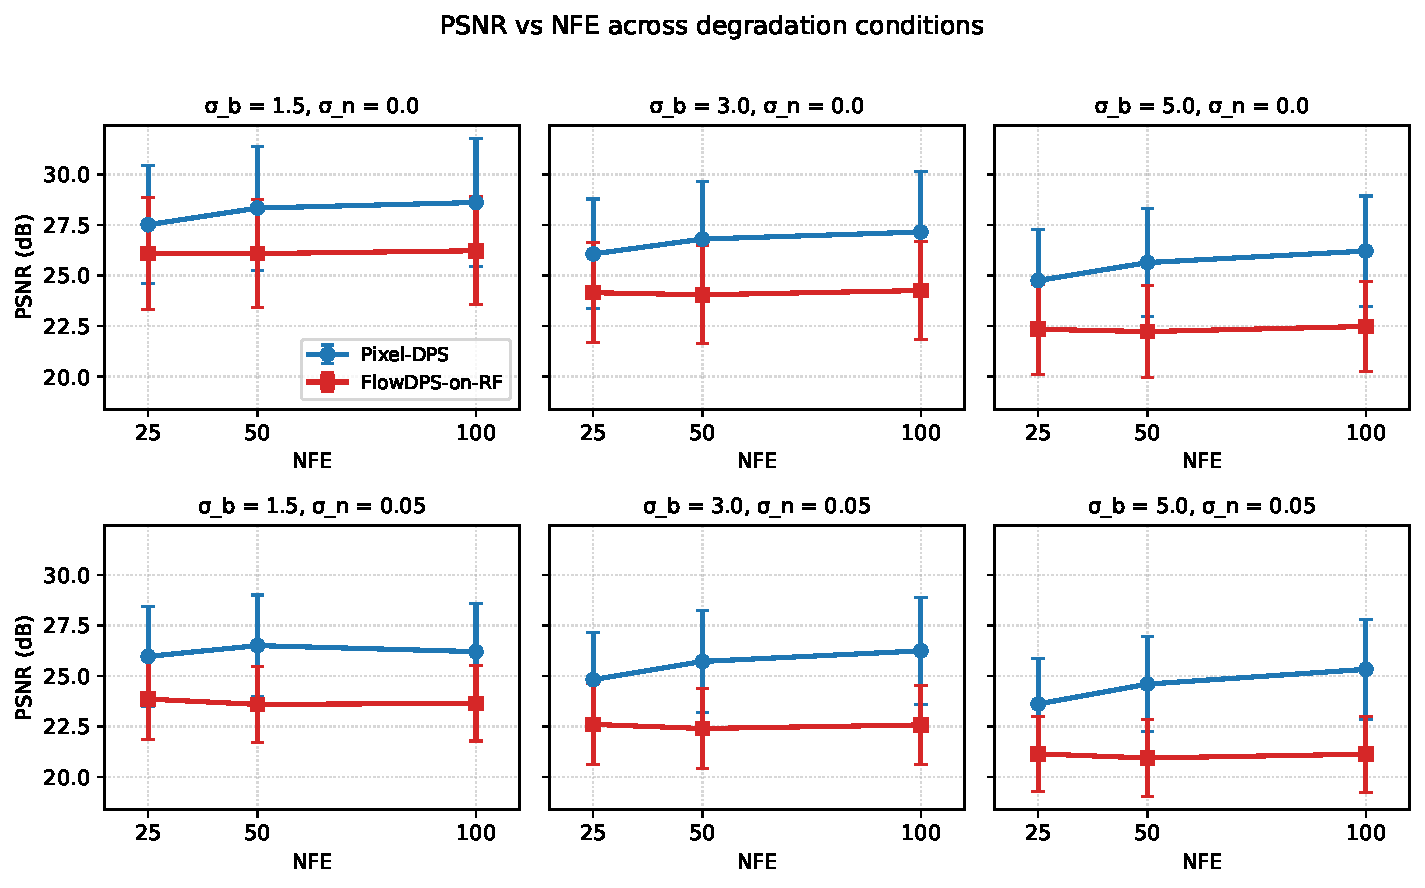
\includegraphics[width=\linewidth]{psnr_vs_nfe}
    \end{column}
    \begin{column}{0.42\linewidth}
      \begin{block}{Key observation}
        FlowDPS-on-RF \textbf{saturates by NFE${=}25$} on this prior.
      \end{block}
      \begin{itemize}
        \item Through NFE${=}200$ FlowDPS gains $<{0.5}$\,dB
        \item Pixel-DPS keeps improving across the whole range
        \item Pixel-DPS is also \textbf{faster per image} on this
              hardware (17.9 vs 23.5 s/img at NFE=100)
      \end{itemize}
    \end{column}
  \end{columns}

  \note{This is the FM-saturation diagnosis that becomes important for
  the Tier-A ablation later. The saturated late-step guidance is what
  the ramp-zeta schedule targets in flowdps_rf_v2.}
\end{frame}

% =====================================================================
\begin{frame}{Operator-mismatch robustness: \textbf{the ordering reverses}}
  \begin{block}{Setup}
    True $A = $ motion blur. Sampler's assumed $A = $ Gaussian.
    Operator misspecification.
  \end{block}

  \vspace{0.3em}
  \begin{table}
    \centering
    \begin{tabular}{lccc}
      \toprule
      & Matched Gaussian & Severe motion mismatch & Drop \\
      \midrule
      \textbf{Pixel-DPS}      & 26.25 dB & 21.3 dB & $-5.0$ dB \\
      \textbf{FlowDPS-on-RF}  & 22.58 dB & 20.1 dB & $\boldsymbol{-2.5}$ \textbf{dB} \\
      Gap (DPS - FlowDPS)     & $+3.67$ dB  & $+0.9$ dB   & narrows \\
      \bottomrule
    \end{tabular}
    \\[0.3em]
    \footnotesize Representative at $\sigma_b{=}3.0$ vs $L{=}35, \theta{=}0^\circ$
  \end{table}

  \begin{alertblock}{The opposite of what the proposal hypothesized}
    The matched-condition $+3.67$ dB Pixel-DPS advantage shrinks to
    $+0.9$ dB. \textbf{FlowDPS-on-RF is relatively more robust to
    operator mismatch.}
  \end{alertblock}

  \note{This is a publishable finding. The deterministic ODE flow seems
  to act as implicit regularization under operator misspecification.
  Practical implication: if you know your operator, use DPS. If you don't,
  consider flow-based posterior sampling.}
\end{frame}

% =====================================================================
\begin{frame}{Posterior diversity: PSNR is not the whole story}
  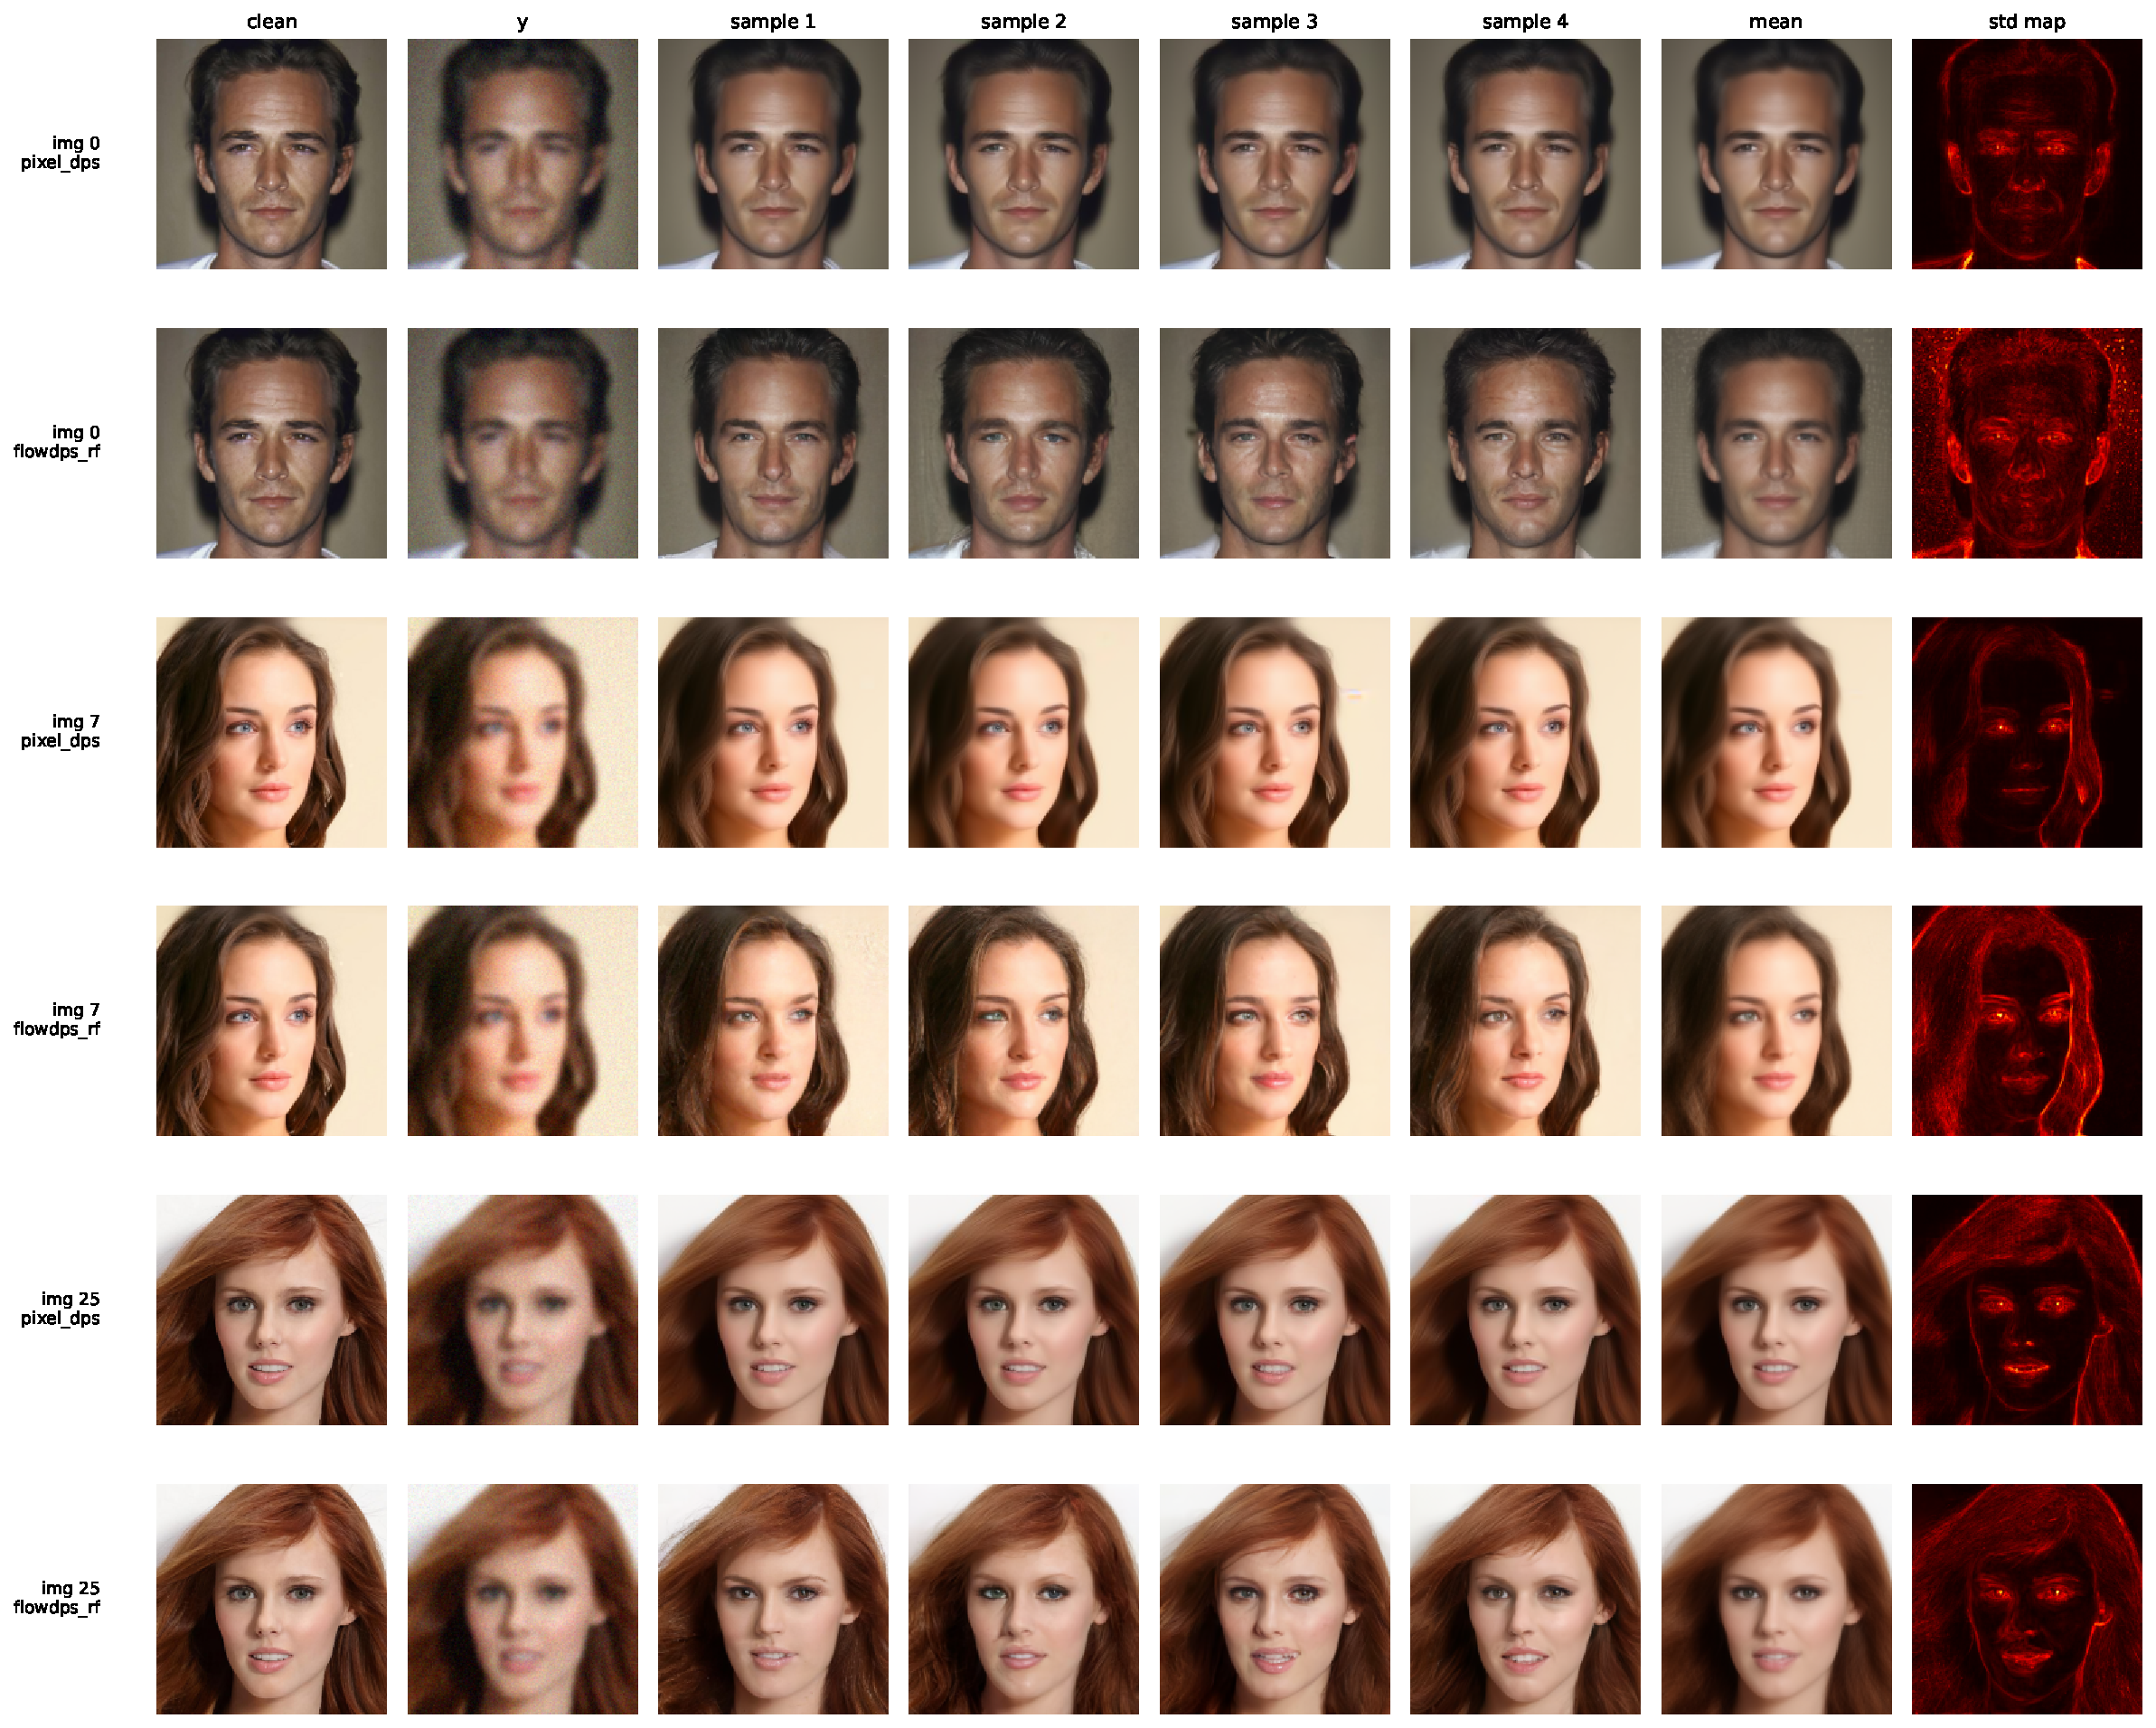
\includegraphics[width=0.95\linewidth]{posterior_diversity}

  \footnotesize 3 images $\times$ 2 methods $\times$ 8 seeds. Held-fixed measurement.

  \note{Pixel-DPS std maps are nearly black - the sampler is collapsing
  to one modal estimate. FlowDPS shows visible diversity in hair, skin,
  micro-features. This is the classical Bayesian critique made measurable.}
\end{frame}

% =====================================================================
\begin{frame}{PSNR vs posterior --- in numbers}
  \begin{table}
    \centering
    \begin{tabular}{lcccc}
      \toprule
      & Single-sample & Mean-of-$N$ & \textcolor{accent}{Pairwise LPIPS} & \textcolor{accent}{std map} \\
      \midrule
      \textbf{Pixel-DPS}     & 29.07 & 29.96 & \textcolor{accent}{0.05}  & \textcolor{accent}{0.012} \\
      \textbf{FlowDPS-on-RF} & 25.57 & 27.72 & \textcolor{accent}{\textbf{0.175}} & \textcolor{accent}{\textbf{0.031}} \\
      \bottomrule
    \end{tabular}
    \\
    \footnotesize $\sigma_b{=}3.0$, $\sigma_n{=}0.05$, NFE${=}50$, $N{=}8$ samples (avg over 3 images)
  \end{table}

  \begin{itemize}
    \item Pixel-DPS produces a \textbf{near-deterministic point estimate}
    \item FlowDPS-on-RF has a \textbf{3.5$\times$ broader posterior}
    \item Pixel-DPS's PSNR advantage is partly a \textbf{point-estimate
          advantage}, not a true posterior-sampling advantage
    \item Posterior-mean gain is larger for FlowDPS-RF
          ($+2.15$ vs $+0.89$ dB) --- larger Bayesian gain from averaging
  \end{itemize}

  \note{From a Bayesian inverse-problems perspective, FlowDPS produces
  a posterior; Pixel-DPS produces a MAP-like point estimate. The right
  method depends on what your downstream application cares about.}
\end{frame}

% =====================================================================
\begin{frame}{Beyond mandatory: 13 ablations under a strict gate}
  \begin{block}{Strict Bonferroni-corrected promotion criterion}
    A method WINS only if:
    (i) mean $\Delta$\,PSNR vs v1 is positive, AND
    (ii) Bonferroni $p<0.05$ in $\geq 4 / 6$ cells.
  \end{block}

  \begin{table}
    \centering
    \small
    \begin{tabular}{llrrl}
      \toprule
      Method & Tier & $\Delta$ (dB) & Sig & Verdict \\
      \midrule
      \texttt{flowdps\_rf\_v2}             & A  & $\boldsymbol{+0.77}$ & $\boldsymbol{6/6}$ & \textcolor{good}{\textbf{WIN}} \\
      \texttt{pixel\_dps\_spectral} matched & B  & $\boldsymbol{+0.46}$ & $\boldsymbol{5/6}$ & \textcolor{good}{\textbf{WIN}} \\
      \texttt{flowdps\_rf\_spectral} matched ($n{=}100$) & B & $\boldsymbol{+0.54}$ & $\boldsymbol{5/6}$ & \textcolor{good}{\textbf{WIN}} \\
      \midrule
      8 other candidates                   & --- & various & 0--$3/6$ & \textcolor{bad}{fail / near-miss} \\
      \bottomrule
    \end{tabular}
  \end{table}

  \begin{itemize}
    \item \textbf{flowdps\_rf\_v2}: EMA-loading bug fix + power-law
          $\zeta$ ramp $\to$ $+0.77$\,dB on FlowDPS-RF
    \item Two spectral wins are the same algorithm on \textbf{both samplers}
  \end{itemize}

  \note{The strict gate is what would separate this from typical
  ablation studies in the literature. Most papers report aggregate
  delta without per-cell correction. 8 candidates would pass a
  permissive criterion but fail our gate - documented as near-misses
  or fails with mechanistic diagnoses.}
\end{frame}

% =====================================================================
\begin{frame}{The paradoxical reversal: our most interesting finding}
  \begin{block}{Spectral-weight algorithm}
    $W(f) = 1 / (1 + \alpha \cdot \mathrm{relu}(\epsilon - |H(f)|))$.
    Downweight residuals where the \emph{assumed} operator's spectrum
    is noise-dominated.
  \end{block}

  \begin{table}
    \centering
    \begin{tabular}{lcc}
      \toprule
      Regime & Pixel-DPS variant & FlowDPS-RF variant \\
      \midrule
      \textbf{Mismatched} (motion meas, gauss assumed)
        & \textcolor{bad}{$-0.18$ dB} & \textcolor{bad}{$-0.20$ dB} \\
      \textbf{Matched} (gauss meas, gauss assumed)
        & \textcolor{good}{$+0.46$ dB $\checkmark$} & \textcolor{good}{$+0.54$ dB $\checkmark$} \\
      \bottomrule
    \end{tabular}
  \end{table}

  \vspace{0.3em}
  \begin{alertblock}{Algorithm-agnostic mechanistic finding}
    Same algorithm, \textbf{opposite verdicts} on adjacent regimes,
    confirmed on both samplers. The mechanism is correctly diagnosed:
    suppression of noise-dominated bands of the \emph{assumed} operator
    helps when assumed${=}$truth and hurts under mismatch.
  \end{alertblock}

  \note{This is the strongest workshop-pitchable finding. A brittle
  ablation would not produce a clean reversal. Confirmed on both
  samplers makes it algorithm-agnostic rather than a single-sampler
  peculiarity.}
\end{frame}

% =====================================================================
\begin{frame}{Eight failed ablations, each with a mechanistic diagnosis}
  \begin{table}
    \centering
    \footnotesize
    \begin{tabular}{lll}
      \toprule
      Method & Failure & Diagnosis \\
      \midrule
      \texttt{pixel\_dps\_v2}      & $-0.66$ dB & v1 $\zeta{=}10$ already near-optimal \\
      \texttt{*\_pigdm} heuristic  & $-13.6$, $-9.8$ dB & L2-norm vs L2-sq convention bug \\
      \texttt{pigdm\_pure} analyt. & $-3.4$ dB & lit: $\Pi$-GDM loses to L2-DPS on Gaussian \\
      \texttt{pixel\_dps\_sched}   & cell-split & optimal $\zeta$ depends on $\sigma_n$ \\
      \texttt{flowdps\_rf\_heun} @ NFE${=}200$ & $-0.17$ dB vs v2 & guidance, not integrator, saturates \\
      \texttt{particle\_dps}       & $-14.8$ dB & path degeneracy: $P_{\mathrm{eff}}{<}1.5$ in 10 steps \\
      \texttt{particle\_dps\_tempered} & $\equiv$ above & SMC without rejuvenation $\to$ SIS \\
      \bottomrule
    \end{tabular}
  \end{table}

  \begin{block}{Negative-result yield}
    All 8 failures match documented failure modes in the literature ---
    we are reproducing known limitations, not encountering novel
    surprises. Each is preserved as code with the diagnosis.
  \end{block}

  \note{Honest framing. Each diagnosis is a useful failure-mode report
  for future re-implementers. The L2-norm vs L2-squared bug is a
  particularly common pitfall.}
\end{frame}

% =====================================================================
\begin{frame}{Discussion: when to use which method}
  \begin{columns}
    \begin{column}{0.5\linewidth}
      \begin{block}{Prefer \textbf{Pixel-DPS} when}
        \begin{itemize}
          \item The forward operator is calibrated
          \item Application wants a sharp point estimate
          \item Modal PSNR is what matters
        \end{itemize}
      \end{block}
    \end{column}
    \begin{column}{0.5\linewidth}
      \begin{block}{Prefer \textbf{FlowDPS-on-RF} when}
        \begin{itemize}
          \item The operator may be misspecified
          \item Downstream Bayesian inference is needed
          \item Posterior diversity matters
        \end{itemize}
      \end{block}
    \end{column}
  \end{columns}

  \vspace{0.3em}
  \begin{block}{Limitations}
    Single dataset (CelebA-HQ-256 faces); two operator families (Gaussian
    + motion); DDRM did not reach competitive PSNR in time;
    $P{=}8$ particles for gradient-free SMC.
  \end{block}

  \begin{block}{Future work}
    Multi-dataset replication; learned $\zeta$ schedule; larger $P$ with
    MCMC rejuvenation; super-resolution and inpainting operators.
  \end{block}
\end{frame}

% =====================================================================
\begin{frame}{Summary of contributions}
  \begin{enumerate}
    \item \textbf{Pixel-space FlowDPS reimplementation} on Liu 2023 RF
          (Kim 2025's code is SD3-only)
    \item \textbf{First quantitative DPS vs FlowDPS comparison} at matched
          resolution + prior on a face dataset
    \item \textbf{Operator-mismatch ordering reversal} quantified
          ($-5$ vs $-2.5$ dB)
    \item \textbf{Posterior-diversity asymmetry} quantified
          (LPIPS 0.05 vs 0.175, $3.5\times$)
    \item \textbf{Three confirmed wins} under strict Bonferroni gate;
          \textbf{paradoxical regime reversal} confirmed on both samplers
    \item \textbf{Eight documented failures} with mechanistic diagnoses
    \item \textbf{Strict-gate ablation methodology} as a rigor improvement
    \item Reproducible pipeline: $10{,}600+$ measurement rows in CSV
  \end{enumerate}

  \begin{block}{Open source}
    \url{https://github.com/adnan821/dps_flowdps}
  \end{block}
\end{frame}

% =====================================================================
\begin{frame}[plain]{}
  \centering
  \vspace{2em}
  {\Huge\bfseries Questions?}

  \vspace{2em}
  {\large Group 13 \\[0.5em]
  Eeman Adnan \quad Muhammad Aslam Adnan \quad Mufaddal Hatim}

  \vspace{2em}
  {\small\url{https://github.com/adnan821/dps_flowdps}}
\end{frame}

\end{document}
